\chapter{Anhang}

\section{Coding Styleguide}
\label{anhang:coding-styleguide}

\subsection{Einleitung}

Die Python-Community legte schon von Beginn an viel Wert auf Lesbarkeit und
Konsistenz von Source Code. Dazu gehört auch ein einheitlicher Code-Stil.  Guido
van Rossum, der Autor von Python, schrieb deshalb seine Vorstellungen von
sauberem Code in einem \textit{Style Guide for Python Code} nieder. Dieser Style
Guide wurde im Jahr 2001 als Python Enhancement Proposal 8 -- kurz PEP8 --
veröffentlicht\footnote{\url{https://python.org/dev/peps/pep-0008/}}.

Der PEP8 Style Guide hat seit dann beinahe universelle Verbreitung gefunden.
Einer der zentralsten Punkte daraus -- die Verwendung von 4 Spaces anstelle von
Tabs -- wird gemäss einem
Analysetool\footnote{\url{http://sideeffect.kr/popularconvention\#python}} in
95\% der Python Projekte auf Github so umgesetzt. Im Rahmen dieser Bachelorarbeit
werden wir daher auch gemäss diesen Richtlinien arbeiten, mit einigen kleinen
Anpassungen.

\subsection{Coding Guidelines}

PEP8 ist in unserer Software verbindlich, mit folgenden Ausnahmen:

\begin{itemize}
	\item Maximale Zeilenlänge ist 109 Zeichen, nicht 79. Heutige Bildschirme sind
		viel grösser, es ergibt keinen Sinn Code umzubrechen, um innerhalb der
		80-Zeichen-Grenze zu bleiben, wenn dadurch der Code weniger gut lesbar wird.
	\item Folgende
		Einrückungsregeln\footnote{\url{http://pep8.readthedocs.org/en/latest/intro.html\#error-codes}}
		in den Code-Checking-Tools können in gewissen Fällen zu schlechter lesbarem
		Code führen und können deshalb ignoriert werden: \textit{E126},
		\textit{E127}, \textit{E128}.
\end{itemize}


\subsection{Future Imports}

Um in einer Python 2 Codebase möglichst gute Vorwärtskompatibilität mit Python 3
zu erreichen, gibt es Backports von neueren Funktionen nach Python 2.7 -- die
sogenannten \textit{Future Imports}. Die empfohlenen Imports für strongTNC sind:

\begin{pythoncode}
from __future__ import print_function, division, absolute_import, unicode_literals
\end{pythoncode}

\noindent Die Beweggründe für diese Liste von Imports sind in einem Blogeintrag
von Stackful.io\footnote{\url{http://stackful-dev.com/quick-tips-on-making-your-code-python-3-ready.html}}
sehr gut erläutert.

Da der Wechsel zu diesen Imports in der aktuellen Codebasis potentiell Bugs
verursachen kann (gerade beim \texttt{unicode\_literals} Import), gilt diese
Empfehlung nur für neue Module. Der Legacy-Code sollte in einem separaten
Refactoring Stück für Stück angepasst werden.


\subsection{Docstrings}

Die meisten Klassen, Methoden und Funktionen sollten mit
Docstrings\footnote{\url{http://legacy.python.org/dev/peps/pep-0257/}}
dokumentiert werden (ausser wenn sie komplett trivial sind).

Docstrings sind mit ReStructuredText formatiert und enden grundsätzlich mit
einer Leerzeile. Wenn ein Docstring nur einen Absatz enthält, kann diese jedoch
weggelassen werden.

\subsubsection*{Beispiel eines Modul-Docstrings:}

\begin{pythoncode}
"""
This module contains DPKG-specific functions for SWID-Tag generation.
"""
\end{pythoncode}

\subsubsection*{Beispiel eines Klassen-Docstrings:}

\begin{pythoncode}
class Foo(object):
    """
    This class is responsible for foo-ing a bar. The resulting foobar object
    can be used for baz.

    Be careful when doing xyz. The reason for this implementation is Lorem
    Ipsum.

    """
    def __init__(self):
        ...
\end{pythoncode}

\subsubsection*{Beispiel eines Funktions- oder Methoden-Docstings:}

\begin{pythoncode}
def myfunc(name, state=None):
    """
    This function does something.

    Args:
        name (unicode or str):
            The name to use.
        state (bool):
            Current state to be in.

    Returns:
        Integer return code. Possible return codes::

            0 -- Success!
            1 -- No good.
            2 -- Try again.

    Raises:
        AttributeError:
            Raised if foo happens.
        RuntimeError:
            Raised if bar is too large.

    A really great idea. A way you might use me is

    >>> print myfunc(name='foo', state=None)
    0

    BTW, this always returns 0. **NEVER** use with :class:`MyPublicClass`.

    """
    return 0
\end{pythoncode}

\subsection{Tools}

\subsubsection{Flake8}

Flake8 (\url{https://flake8.readthedocs.org/en/2.0/}) verbindet das Style
Checking Tool pep8\footnote{\url{https://pypi.python.org/pypi/pep8}} mit dem
Static Code Analysis Tool
pyflakes\footnote{\url{https://pypi.python.org/pypi/pyflakes}}. Für unser
Projekt kann folgende Konfiguration (\texttt{~/.config/flake8}) verwendet
werden:

\begin{inicode}
[flake8]
ignore = E126,E127,E128
max-line-length = 109
\end{inicode}

\subsubsection{Pytest}

Zum von uns verwendeten Testing-Framework
Pytest\footnote{\url{http://pytest.org/}} gibt es ein PEP8 Plugin. Wird dieses
aktiviert, werden Style Guide Violations als fehlerhafte Tests gewertet.
Folgende Konfiguration wird dafür in \texttt{pytest.ini} verwendet:

\begin{inicode}
[pytest]
addopts = --pep8
pep8ignore =
    *.py E126 E127 E128
    setup.py ALL
    settings.py ALL
    urls.py ALL
    */migrations/* ALL
    */tests/* ALL
pep8maxlinelength = 109
\end{inicode}


\section{Git Guidelines}
\label{ref:git-guidelines}

Nachfolgend ein paar Regeln zum Umgang mit Git, mit dem Ziel eine möglichst
saubere History zu haben.

\subsection{Commit-Messages}

\begin{itemize}
	\item ...beginnen mit einem Grossbuchstaben
	\item ...sind in Englisch verfasst
	\item ...enthalten keine Typos
	\item ...enthalten keine Smileys
	\item ...sind kurz und prägnant
	\item ...enthalten keine relativen Ticket-Referenzen wie \texttt{refs \#1},
		nur absolute Referenzen wie \texttt{fixes user/repo\#2}. Die
		Referenzen sollten im Beschreibungstext stehen, nicht in der ersten Zeile.
	\item ...sind in past tense geschrieben (\textit{fixed bug} statt \textit{fix
		bug})
\end{itemize}

\noindent Generell sollte die erste Zeile einer Commit Message in höchstens 72
Zeichen\footnote{\url{http://tbaggery.com/2008/04/19/a-note-about-git-commit-messages.html}}
die Änderungen zusammenfassen. Weitere Erläuterungen sollten durch eine
Leerzeile getrennt werden.

\paragraph{Beispiel:} ~\\

\begin{textcode}
Capitalized, short (72 chars or less) summary

More detailed explanatory text, if necessary.  Wrap it to about 72
characters or so.  In some contexts, the first line is treated as the
subject of an email and the rest of the text as the body. The blank
line separating the summary from the body is critical (unless you omit
the body entirely); tools like rebase can get confused if you run the
two together.

Further paragraphs come after blank lines.

- Bullet points are okay, too

- Typically a hyphen or asterisk is used for the bullet, followed by a
  single space, with blank lines in between, but conventions vary here

- Use a hanging indent
\end{textcode}

\subsection{History}

\subsubsection{Rewriting / Reordering / Squashing}

Die Git History sollte sauber gehalten werden. Während der Entwicklung ist es
kein Problem, wenn man viele und häufige Commits macht, aber vor einem
Merge/Rebase in den Hauptcode sollten die Commits sinnvoll reduziert (squashed)
werden. 

Alles zum Verändern der Git History findet sich hier:\\
\url{http://git-scm.com/book/en/Git-Tools-Rewriting-History}

\subsubsection{Pulling}

Beim \texttt{git pull} ist es sinnvoll, immer den \texttt{-{}-rebase} Parameter zu
verwenden. Bei einem Konflikt durch neue Remote Commits wird dann nämlich lokal
rebased statt merged. Da der lokale Code noch nicht publiziert wurde, ist dies
unbedenklich. Ein Rebase-Konflikt kann bei Problemen jederzeit mit \texttt{git
rebase -{}-abort} abgebrochen werden.

\subsubsection{Force Pushing}

Während der Entwicklungsphase in einem Branch ist es kein Problem wenn man
geänderte History mit \texttt{git push -{}-force} pushed, im \texttt{master}
Branch sollte das jedoch nur in äussersten Ausnahmesituationen geschehen.

\subsubsection{Merge / Rebase}

Ist ein Pull Request abgeschlossen, sollte er vor einem Merge gegen den
\texttt{master}-Branch rebased werden. Dies verhindert Konflikte und ermöglicht
ein \textit{fast-forward merge}, wodurch kein Merge Commit entsteht:

\begin{bashcode}
git checkout master
git pull --rebase
git checkout <featurebranch>
git rebase master
# fix potential conflicts
# squash commits with git rebase <latest-master-commit>
git push --force origin <featurebranch>
\end{bashcode}

\noindent Danach sollte der Pull Request sofort gemerged werden:

\begin{bashcode}
git checkout master
git merge --ff-only <featurebranch>
git push
\end{bashcode}


\section{Workflow}

\subsection{Ablauf}

Nachfolgend der Workflow einer Code-Änderung:

\begin{enumerate}
	\item Ticket wird im Github Issue Tracker erstellt und jemandem zugewiesen.
	\item Der zuständige Entwickler erstellt einen Feature Branch und entwickelt
		darin den benötigten Code.
	\item Wenn der entwickelte Code sich im strongTNC Repository befindet, kann
		der Issue in ein Pull Request umgewandelt werden (\ref{workflow:hub}).
		Ansonsten einen separaten Pull Request erstellen und darin auf den Issue
		verweisen (\texttt{refs user/repo\#issue}).
	\item Code wird von jemandem reviewed. Korrekturen werden in den Branch
		pushed.
	\item Commits werden wenn sinnvoll reduziert.
	\item Rebase des Branches gegen \texttt{master}.
	\item Merge in \texttt{master} via Kommandozeile.
	\item Ticket mit Referenz auf relevante Commits schliessen.
\end{enumerate}

\subsection{Umwandeln von Issues in Pull Requests}
\label{workflow:hub}

Mit dem Kommandozeilen-Tool hub\footnote{\url{https://github.com/github/hub}}
kann ein Issue in ein Pull Request umgewandelt werden:

\begin{bashcode}
git checkout <featurebranch>
git push origin <featurebranch>
hub pull-request -b tnc-ba/strongTNC:master -i <issue-number> -h <featurebranch>
\end{bashcode}


\section{Definition of Done}
\label{DefinitionOfDone}

Ein Task gilt als abgeschlossen, wenn folgende Punkte erfüllt sind:

\begin{itemize}
	\item Alle Arbeiten gemäss Task-Beschreibung wurden ausgeführt.
	\item Der Code wurde auf Github in einen Feature Branch committed.
	\item Der Code wurde von einem Teammitglied reviewed.
	\item Der Code ist sinnvoll kommentiert, Docstrings für Funktionen und Klassen sind vorhanden.
	\item Flake8 zeigt keine Fehler oder Warnungen.
	\item Tests existieren wo sinnvoll. Die Testsuite läuft erfolgreich durch.
	\item Dokumentation wurde nachgeführt.
	\item Der Feature Branch wurde in den Master Branch gemerged.
	\item Die benötigte Arbeitszeit wurde erfasst.
\end{itemize}

\section{strongTNC Deployment Manual}
\label{anhang:deployment-manual}

Due to security- and performance-considerations, strongTNC should never be
deployed into production using the \texttt{./manage.py runserver} command.
Instead, a proper WSGI Webserver should be used, and all debug settings should
be turned off.

\textbf{Warning: Never deploy strongTNC in production without using SSL/TLS to
secure your connections, especially if you use the API.}

The following how-to assumes you're using Ubuntu or a similar Linux
distribution, but the basic concepts can be applied to any Linux distribution.

(Note: If you just want to try strongTNC, you can also use the automatially
configured testing VMs. See \texttt{vm/README.rst} for more information.)

\subsection*{Install the base system}

Set up your base Ubuntu system. Make sure all the packages are up to date.

\subsection*{Install required packages}

Install the dependencies for strongTNC:

\begin{bashcode}
sudo apt-get install wget build-essential apache2 libapache2-mod-wsgi python2.7 \
    python2.7-dev python-pip python-virtualenv libxml2-dev libxslt1-dev
\end{bashcode}

If you want to use MySQL instead of SQLite, you need a few additional
dependencies:

\begin{bashcode}
sudo apt-get install mysql-server mysql-client libmysqlclient-dev
\end{bashcode}

\subsection*{Create directories}

\begin{bashcode}
sudo mkdir /var/www/strongTNC /etc/strongTNC
sudo chown $(whoami):www-data /var/www/strongTNC /etc/strongTNC
sudo chmod 775 /var/www/strongTNC /etc/strongTNC
\end{bashcode}

\subsection*{Download current strongTNC release}

Download the current snapshot of the master branch from Github:

\begin{bashcode}
cd /tmp
wget https://github.com/strongswan/strongTNC/archive/master.tar.gz
tar xfvz master.tar.gz
mv strongTNC-master/* /var/www/strongTNC/
\end{bashcode}

If you want you could also use git to clone the repository.

\subsection*{Install Python dependencies}

The recommended way to install the Python dependencies is to put them in a
Virtualenv\footnote{\url{http://virtualenv.readthedocs.org/}}.

\begin{bashcode}
cd /var/www/strongTNC
virtualenv --no-site-packages VIRTUAL
VIRTUAL/bin/pip install -U -r requirements.txt
\end{bashcode}

If you use MySQL, you need an additional Python package:

\begin{bashcode}
VIRTUAL/bin/pip install -U MySQL-python
\end{bashcode}

\subsection*{strongTNC configuration}

Copy the sample configuration to /etc:

\begin{bashcode}
cp /var/www/strongTNC/config/settings.sample.ini /etc/strongTNC/settings.ini
cd /etc/strongTNC/
sudo chown $(whoami):www-data settings.ini
sudo chmod 640 settings.ini
\end{bashcode}

Now edit the configuration file with your favorite text editor. First of all,
update the database configuration. If you want to use SQLite, set them to the
following values:

\begin{bashcode}
DJANGO_DB_URL = sqlite:////var/www/strongTNC/django.db
STRONGTNC_DB_URL = sqlite:////var/www/strongTNC/ipsec.config.db
\end{bashcode}

For MySQL, use the following values:

\begin{bashcode}
DJANGO_DB_URL = mysql://strongtnc:<mysql-password>@127.0.0.1/strongtnc_django
STRONGTNC_DB_URL = mysql://strongtnc:<mysql-password>@127.0.0.1/strongtnc_data
\end{bashcode}

(Choose a secure password and remember it for later, when we create the MySQL
user!)

Now you need to set a value for \texttt{SECRET\_KEY}, which is used by Django to
encrypt all kinds of stuff. A way to generate such a key is the following code
snippet:

\begin{bashcode}
dd if=/dev/urandom bs=128 count=1 2>/dev/null | base64 -w 175
\end{bashcode}

Then set \texttt{ALLOWED\_HOSTS} to a list of hostnames that will be allowed to
serve strongTNC, e.g.

\begin{bashcode}
ALLOWED_HOSTS = 127.0.0.1,strongtnc.example.org
\end{bashcode}

If you enable SSL/TLS for your setup (you really should!), enable secure CSRF
cookies:

\begin{bashcode}
CSRF_COOKIE_SECURE = 1
\end{bashcode}

You should also take a look at the \texttt{[admins]} section and add your name
and e-mail address there.

\subsection*{Set up database}

\subsubsection*{SQLite}

If you're using SQLite, all you need to do is changing the database permissions:

\begin{bashcode}
cd /var/www/strongTNC/
sudo chgrp www-data django.db ipsec.config.db
sudo chmod 660 django.db ipsec.config.db
\end{bashcode}

\subsubsection*{MySQL}

First, log in to the MySQL console with the root user:

\begin{bashcode}
mysql -u root -p
\end{bashcode}

Create the required databases:

\begin{sqlcode}
mysql> CREATE DATABASE strongtnc_django CHARACTER SET utf8 COLLATE utf8_unicode_ci;
mysql> CREATE DATABASE strongtnc_data CHARACTER SET utf8 COLLATE utf8_unicode_ci;
\end{sqlcode}

Create a new user (make sure to replace \texttt{<password>} with the previously
chosen MySQL password):

\begin{sqlcode}
mysql> GRANT ALL PRIVILEGES ON strongtnc_django.* TO strongtnc@localhost
-> IDENTIFIED BY '<password>';
mysql> GRANT ALL PRIVILEGES ON strongtnc_django.* TO strongtnc@localhost
-> IDENTIFIED BY '<password>';
\end{sqlcode}

Create the necessary schema in your database:

\begin{bashcode}
cd /var/www/strongTNC/
VIRTUAL/bin/python manage.py syncdb --database=meta --noinput
VIRTUAL/bin/python manage.py syncdb --database=default --noinput
\end{bashcode}

\subsection*{Collect static files}

Run the following command to collect all static files in a single directory:

\begin{bashcode}
cd /var/www/strongTNC/
VIRTUAL/bin/python manage.py collectstatic --noinput
\end{bashcode}

\subsection*{Apache configuration}

Write the following configuration to \texttt{/etc/apache2/sites-available/strongTNC}

\begin{apachecode}
WSGIPythonPath /var/www/strongTNC:/var/www/strongTNC/VIRTUAL/lib/python2.7/site-packages

NameVirtualHost *:80
<VirtualHost *:80>
    RewriteEngine On
    RewriteCond %{HTTPS} off
    RewriteRule (.*) https://%{HTTP_HOST}%{REQUEST_URI}
</VirtualHost>

<VirtualHost _default_:443>
    # The ServerName directive sets the request scheme, hostname and port that
    # the server uses to identify itself. This is used when creating
    # redirection URLs. In the context of virtual hosts, the ServerName
    # specifies what hostname must appear in the request's Host: header to
    # match this virtual host. For the default virtual host (this file) this
    # value is not decisive as it is used as a last resort host regardless.
    # However, you must set it for any further virtual host explicitly.
    #ServerName strongtnc.example.com

    SSLEngine on
    SSLCertificateFile /etc/apache2/ssl/strongtnc.crt
    SSLCertificateKeyFile /etc/apache2/ssl/strongtnc.key
    SSLProtocol all -SSLv2 -SSLv3
    SSLHonorCipherOrder on
    SSLCompression off
    SSLCipherSuite "EECDH+ECDSA+AESGCM EECDH+aRSA+AESGCM EECDH+ECDSA+SHA384 \
        EECDH+ECDSA+SHA256 EECDH+aRSA+SHA384 EECDH+aRSA+SHA256 EECDH+aRSA+RC4 \
        EECDH EDH+aRSA RC4 !aNULL !eNULL !LOW !3DES !MD5 !EXP !PSK !SRP !DSS"
    Header add Strict-Transport-Security "max-age=15768000"

    ServerAdmin webmaster@localhost
    DocumentRoot /var/www/strongTNC

    <Directory /var/www/strongTNC>
        <Files wsgi.py>
            Order deny,allow
            Allow from all
        </Files>
        Options -Indexes
    </Directory>

    WSGIScriptAlias / /var/www/strongTNC/config/wsgi.py
    Alias /static/ /var/www/strongTNC/static/

    WSGIPassAuthorization On

    ErrorLog ${APACHE_LOG_DIR}/error.log
    CustomLog ${APACHE_LOG_DIR}/access.log combined
</VirtualHost>

# vim: syntax=apache ts=4 sw=4 sts=4 sr noet
\end{apachecode}

Then disable the default configuration and enable strongTNC:

\begin{bashcode}
sudo a2dissite 000-default
sudo a2ensite strongTNC
\end{bashcode}

Enable necessary plugins and create ssl directory:

\begin{bashcode}
sudo a2enmod ssl rewrite headers
sudo mkdir /etc/apache2/ssl
\end{bashcode}

Copy your TLS certificate and the private key to \texttt{/etc/apache2/ssl}. If
you want to create self-signed certificates, execute the following command:

\begin{bashcode}
sudo openssl req -x509 -nodes -sha256 -days 365 -newkey rsa:3072 -utf8 \
    -keyout /etc/apache2/ssl/strongtnc.key -out /etc/apache2/ssl/strongtnc.crt
\end{bashcode}

Make sure the permissions are restrictive:

\begin{bashcode}
sudo chown root:root /etc/apache2/ssl/*
sudo chmod 400 /etc/apache2/ssl/*
\end{bashcode}

Now restart Apache and strongTNC should be up and running!

\begin{bashcode}
sudo service apache2 restart
\end{bashcode}

\subsection*{Create default users}

In order to be able to login into strongTNC, you need to set a password for a
readonly user and an admin user.

\begin{bashcode}
cd /var/www/strongTNC/
VIRTUAL/bin/python manage.py setpassword
\end{bashcode}

Visit \texttt{http://yourserver/} to log in.


\section{strongTNC REST API Konzept}
\label{REST:api-konzept}
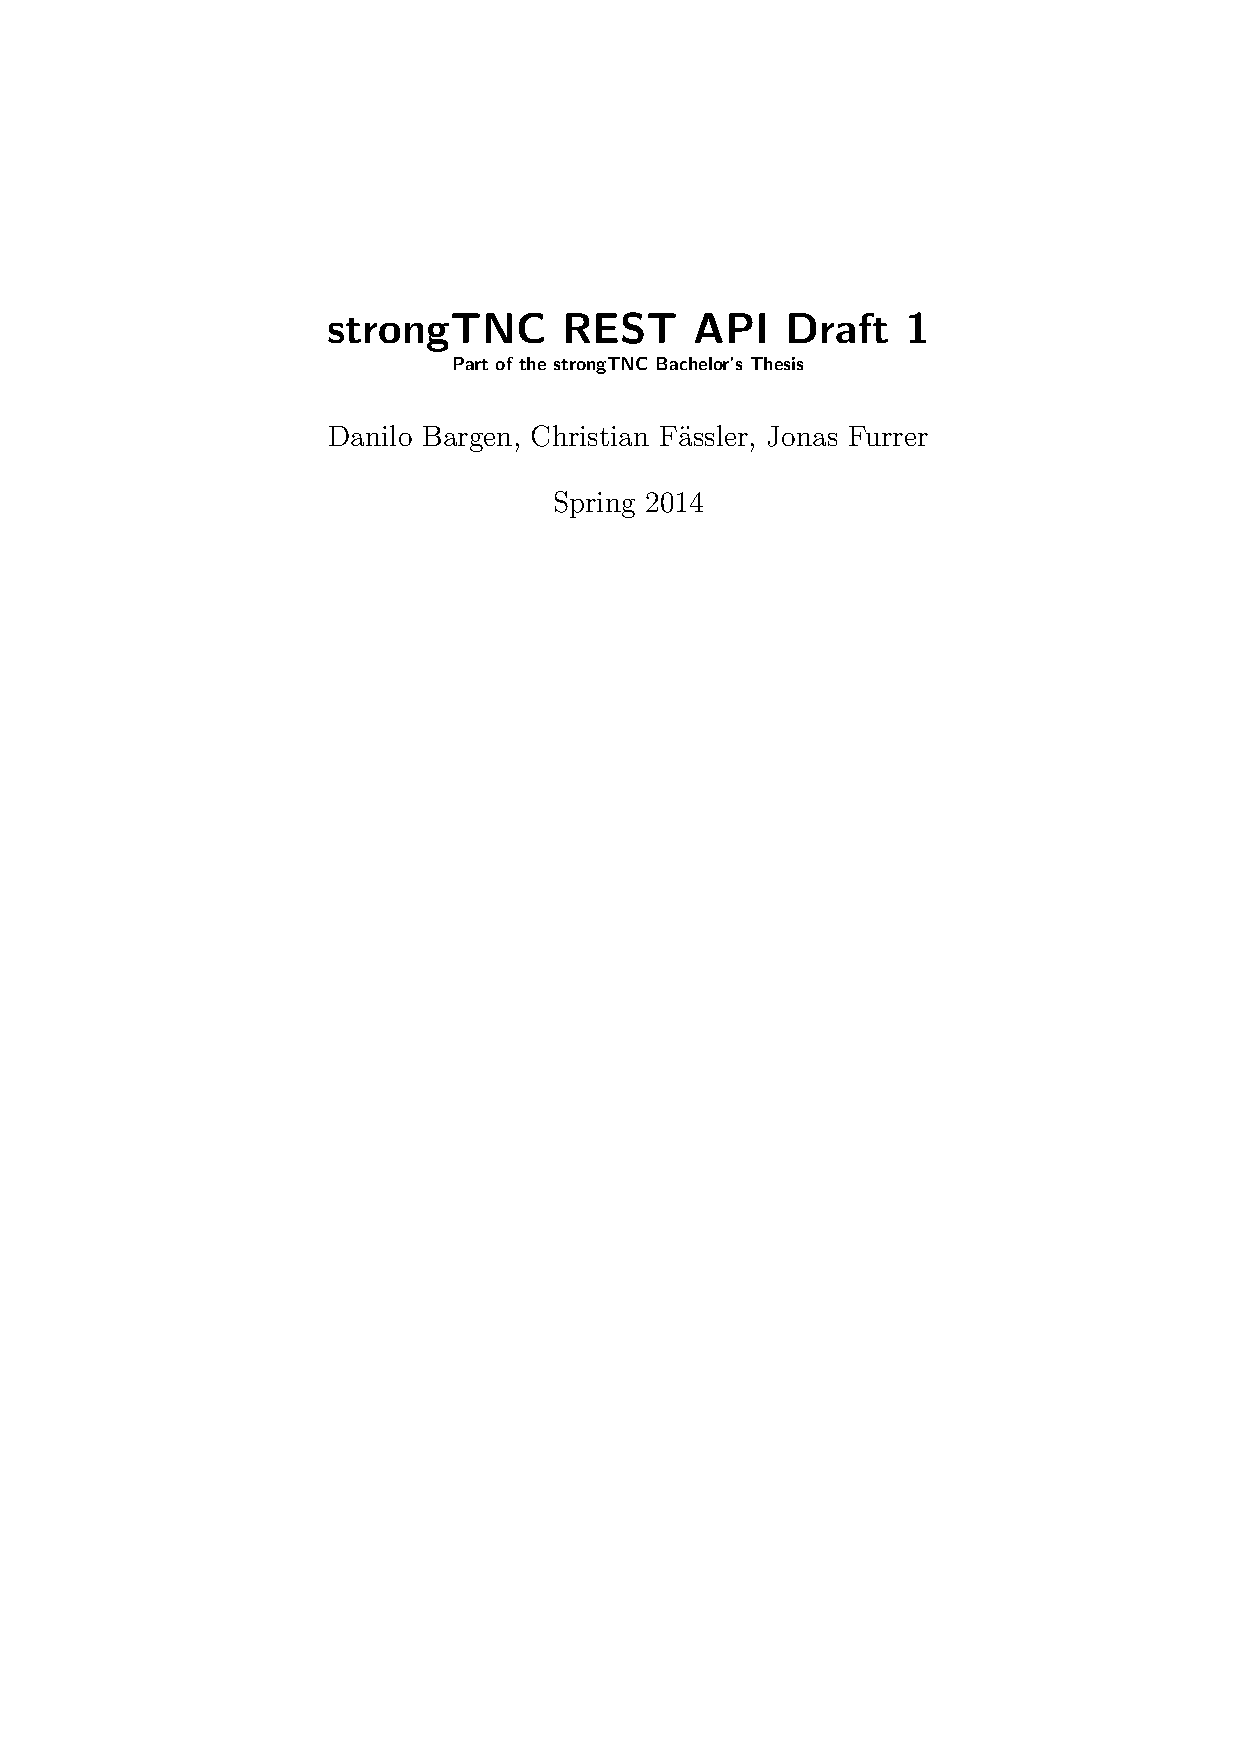
\includepdf[height=\textheight,pages={-},offset=0mm -5mm, frame=true]{other_documents/REST-interface.pdf}

\section{SWID Measurement Endpoint REST Manual}
\label{REST:swid-measurement-manual}
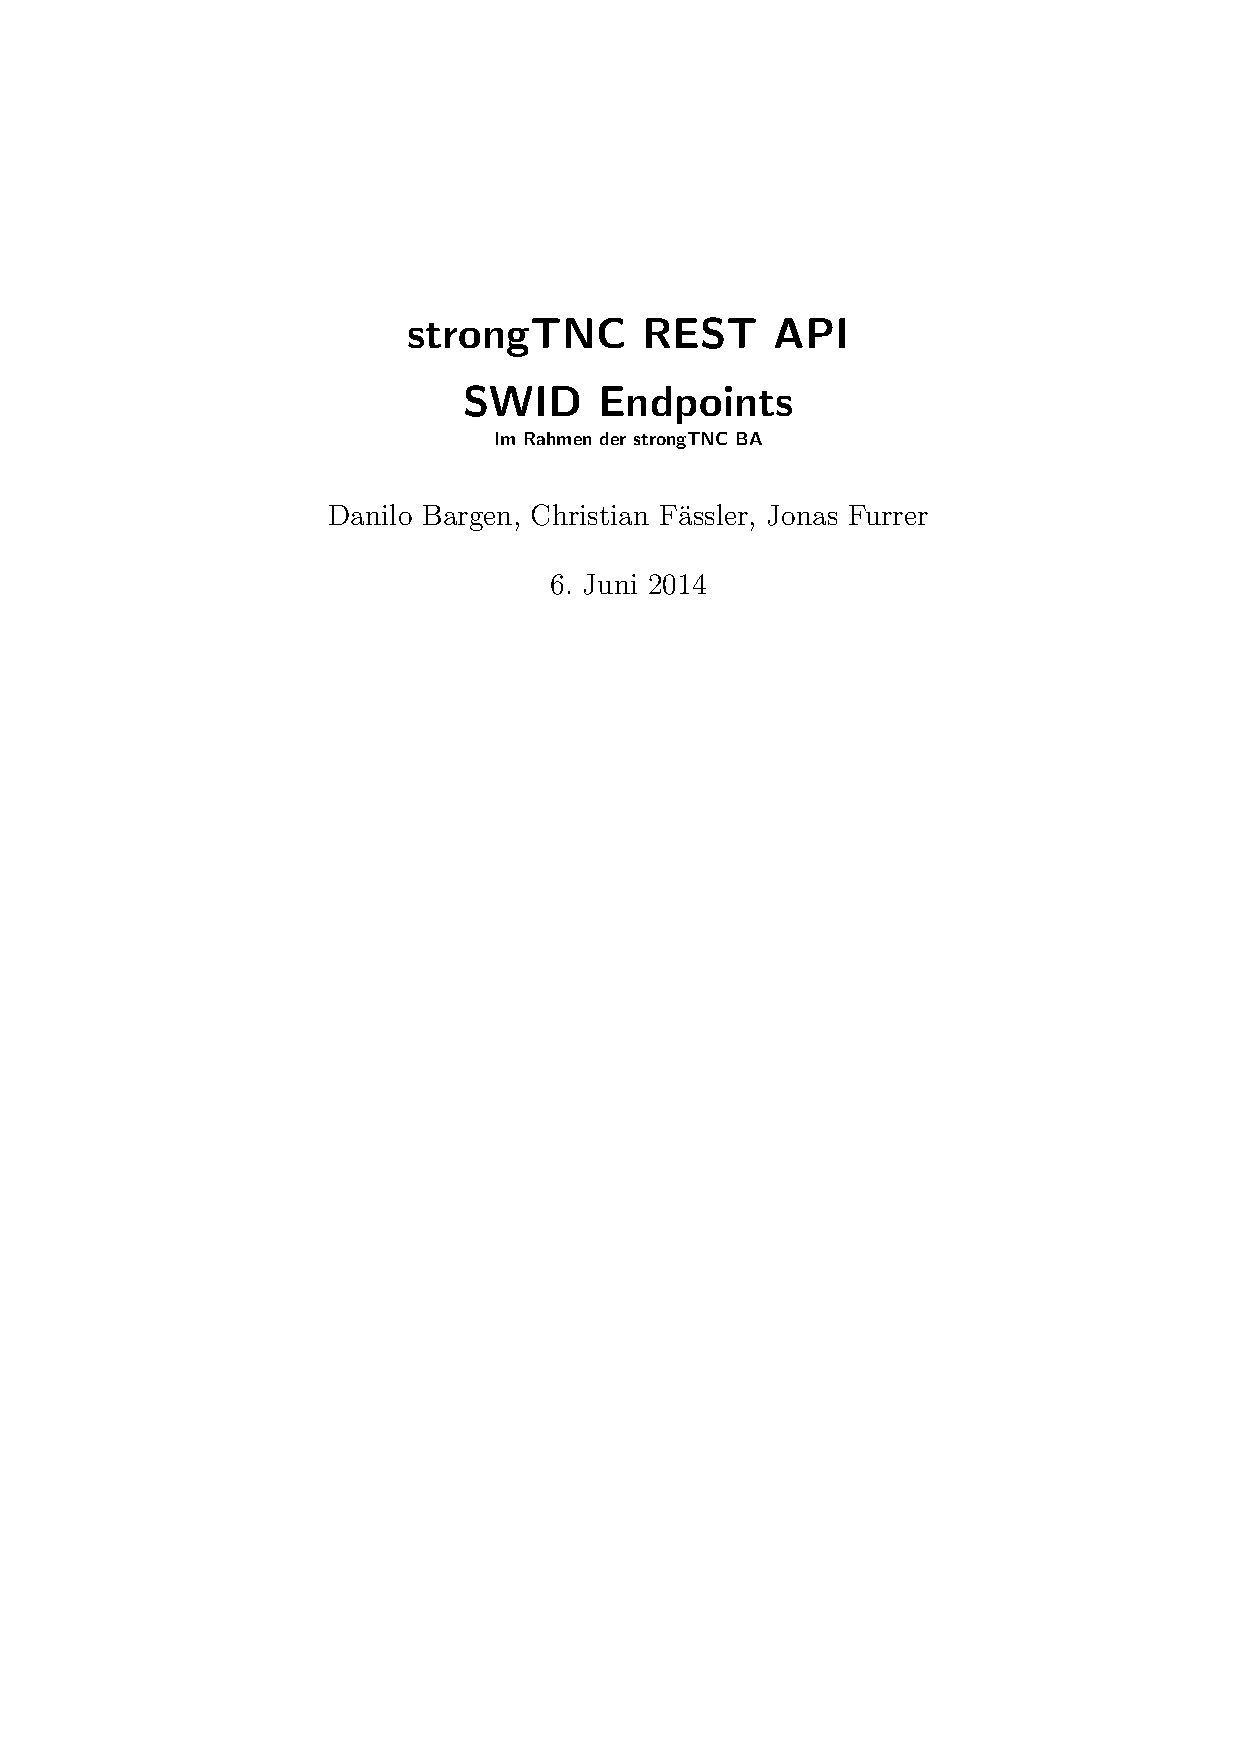
\includepdf[height=\textheight,pages={-},offset=0mm -5mm, frame=true]{other_documents/swid-measurement-manual.pdf}

\section{Zeitplanung}
\label{anhang:zeitplanung}
\subsection{Iterationen / Phasen}

Die zur Verfügung stehende Arbeitszeit wurde in sechs Iterationen zu jeweils
zwei Wochen und noch zwei Iterationen zu je einer Woche eingeteilt. Anhand der
bekannten Arbeitspaketen aus der Aufgabenstellung haben wir das Projekt in zwei
Phasen aufgeteilt. \\
In der ersten Phase haben wir uns den Pflichtteilen der Aufgabenstellung
angenommen. Die wesentlichen Ziele waren die Behebung der bereits bekannten Bugs
sowie die Implementation einer ersten Version des SWID Generators und der
entsprechenden Erweiterung der strongTNC App. \\
In der zweiten Phase konzentrierten wir uns in die Ausarbeitung des Konzeptes
strongTNC API, sowie architektonische Konzepte, die nicht Bestandteil der
Aufgabenstellung waren (siehe \autoref{analyse:soll-situation})

Das Ziel dieser Trennung war die Minimierung von Risiken, die erste Phase
erlaubte es Prototypen zu implementieren und die nötige Spezifikation zu
liefern, welche für die Integration in die strongSwan Infrastruktur nötig war.
Der detailierte Zeitplan ist im Anhang zu finden (\autoref{anhang:zeitplanung}).

\subsection{Zeiterfassung}

Während der gesamten Laufzeit der Arbeit haben wir für jeden Github Issue den
Zeitaufwand geschätzt und zusammen mit dem effektiven Aufwand in einem Google
Docs Spreadsheet festgehalten. Dies ermöglicht detaillierte Auswertungen der
benötigten Zeit sowie der Schätzungsgenauigkeit.

\subsubsection{Aufwand}

Der Aufwand pro Iteration stieg im Verlauf der Wochen stetig an (Abbildung
\ref{zeitanalyse:total}). In den ersten Iterationen war der Gesamtaufwand
geringer als später, weil eines unserer Teammitglieder unfallbedingt zwei Wochen
ausfiel. Dies ist auch gut in der Abbildung \ref{zeitanalyse:total-pro-person}
ersichtlich. \\
In der siebten Iteration stieg der Aufwand signifikant an, da wir die Feiertage
um Auffahrt nutzten um an dieser Arbeit weiterzuarbeiten. \\
Nach der sechsten Iteration war an der HSR Unterrichtsschluss, entsprechend
waren für die letzten zwei Iterationen mehr Zeit eingeplant. Die effektiv
geleistete Zeit überstieg diese jedoch noch stark.

Wie man in Abbildung \ref{zeitanalyse:tickets} sieht, korrelliert der geleistete
Aufwand korrelliert mit der Anzahl der geschlossenen Tickets pro Iteration. Mit
Abstand die meisten Tickets wurden in der siebten Iteration geschlossen. Dies
liegt einerseits am höheren Arbeitsaufwand, andererseits daran dass wir in
dieser Iteration mit intensivem Testen von strongTNC begonnen haben, was einige
neuen Bugs zu Tage brachte.

\subsubsection{Schätzungsgenauigkeit}

In der Abbildung \ref{zeitanalyse:abweichung} sieht, wurde die Zeitschätzung in
der ersten Hälfte der Arbeit immer besser, während sie sich in der zweiten Hälfte
wieder verschlechterte. \\
Die anfänglich hohe negative Abweichung liegt einerseits an unserer sehr
konservativen Schätzungsweise, andererseits daran dass aufgrund des Unfalls von
Danilo Bargen weniger Stunden geleistet wurden, als ursprünglich geschätzt
wurden. \\
In der Hälfte der Arbeit verbesserten sich die Schätzungen, in den letzten
Wochen verschlechterte sie sich jedoch wieder. Dies ist einerseits auf den
erhöhten Arbeitsaufwand zurückzuführen, andererseits auf den unterschätzten
Dokumentationsaufwand.

\begin{sidewaysfigure}
	\begin{minipage}[t]{0.45\textwidth}
		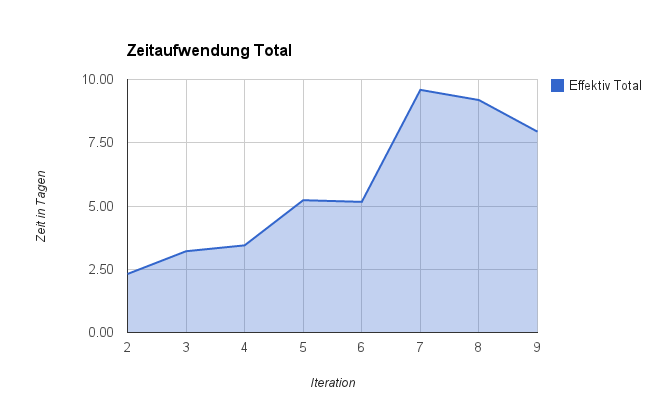
\includegraphics[width=\linewidth]{images/zeitplanung/chart_1}
		\caption{Zeitaufwendung Total}
		\label{zeitanalyse:total}
	\end{minipage}
	\hspace{\fill}
	\begin{minipage}[t]{0.45\textwidth}
		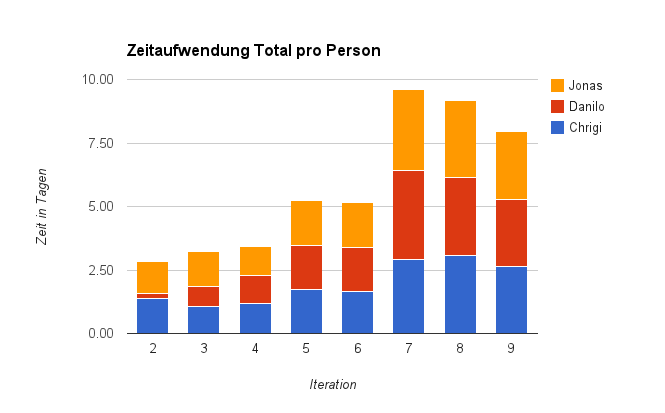
\includegraphics[width=\linewidth]{images/zeitplanung/chart_2}
		\caption{Zeitaufwendung Total pro Person}
		\label{zeitanalyse:total-pro-person}
	\end{minipage}

	\vspace{2cm}

	\begin{minipage}[t]{0.45\textwidth}
		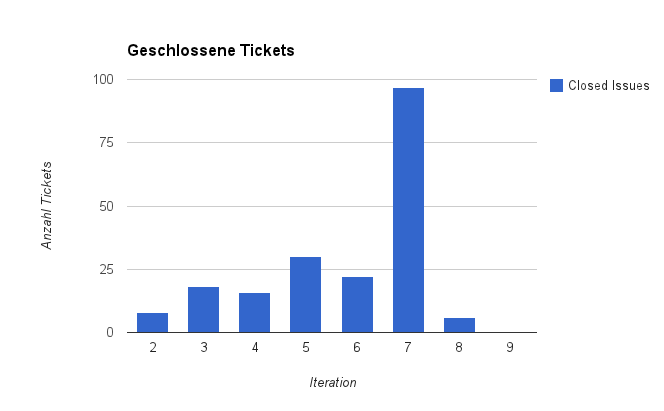
\includegraphics[width=\linewidth]{images/zeitplanung/chart_3}
		\caption{Geschlossene Tickets}
		\label{zeitanalyse:tickets}
	\end{minipage}
	\hspace{\fill}
	\begin{minipage}[t]{0.45\textwidth}
		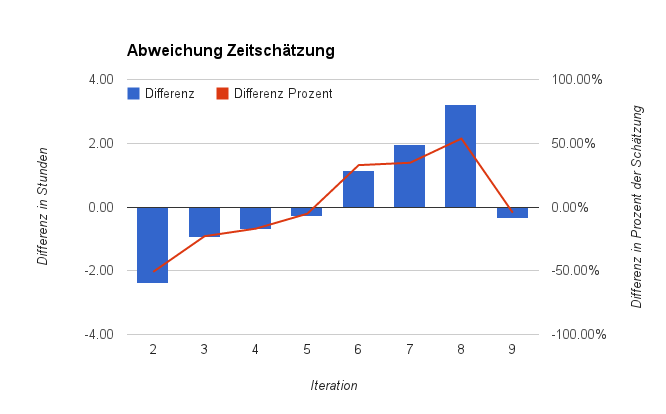
\includegraphics[width=\linewidth]{images/zeitplanung/chart_4}
		\caption{Abweichung Zeitschätzung}
		\label{zeitanalyse:abweichung}
	\end{minipage}

\end{sidewaysfigure}

\begin{sidewaysfigure}

	\begin{minipage}[t]{0.9\textwidth}
		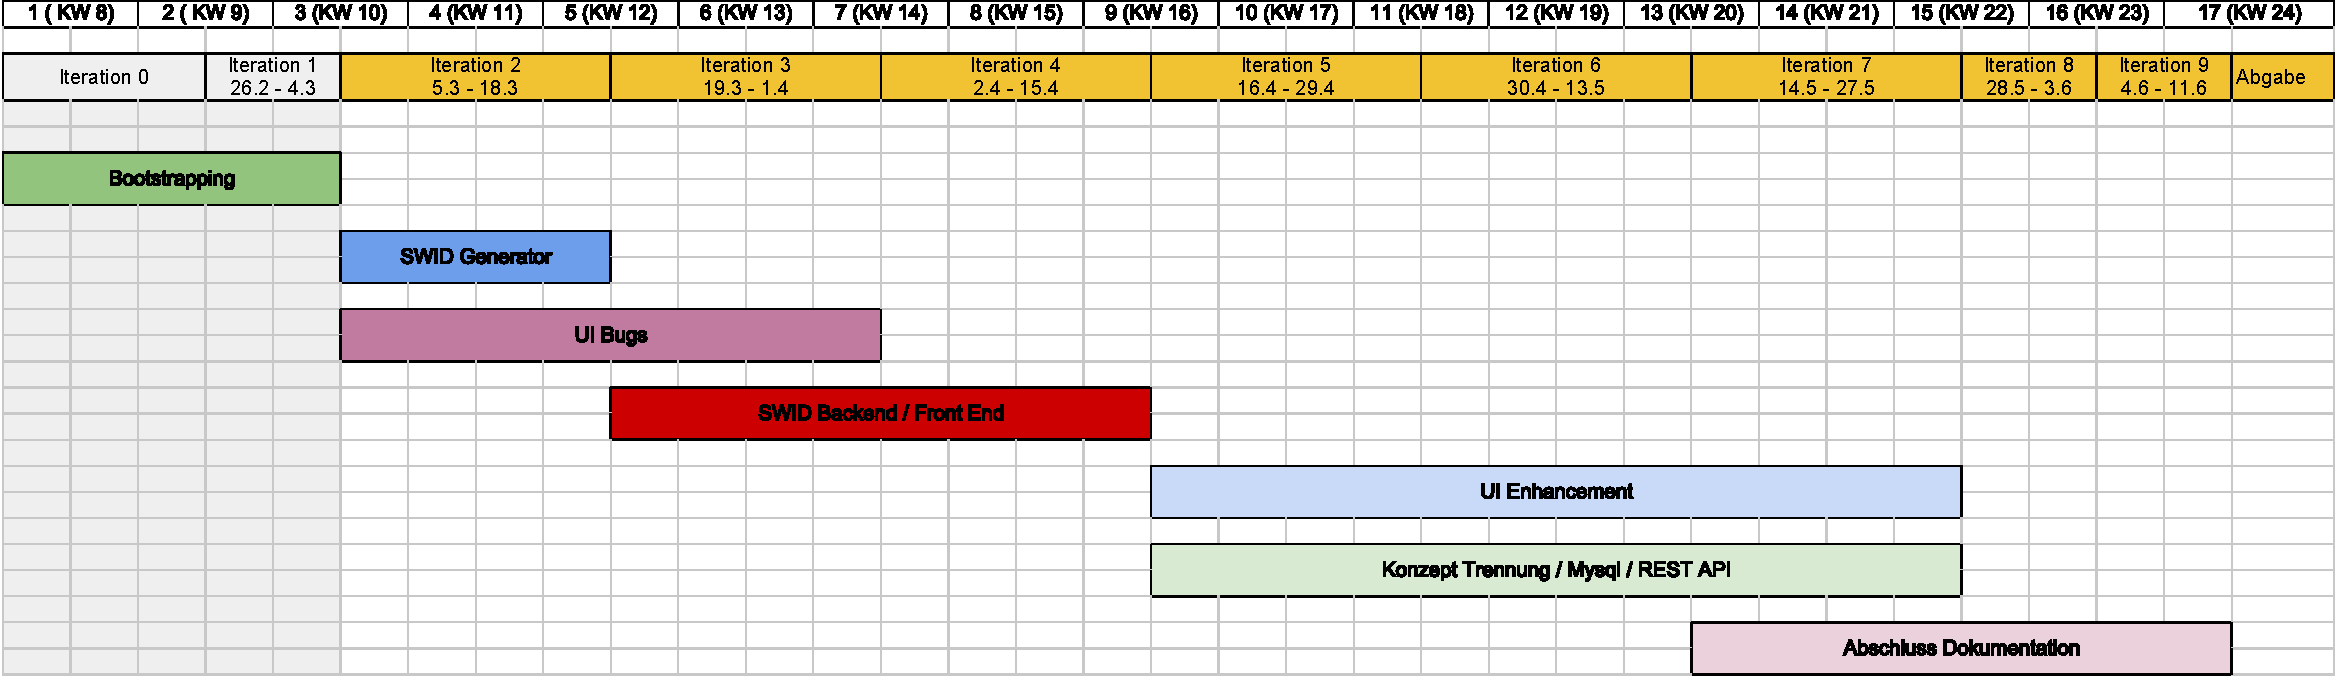
\includegraphics[width=\linewidth]{images/zeitplanung/iteration_1}
		\caption{Zeitplanung zu Beginn der Arbeit}
		\label{zeitanalyse:vorher}
	\end{minipage}

	\vspace{2cm}

	\begin{minipage}[t]{0.9\textwidth}
		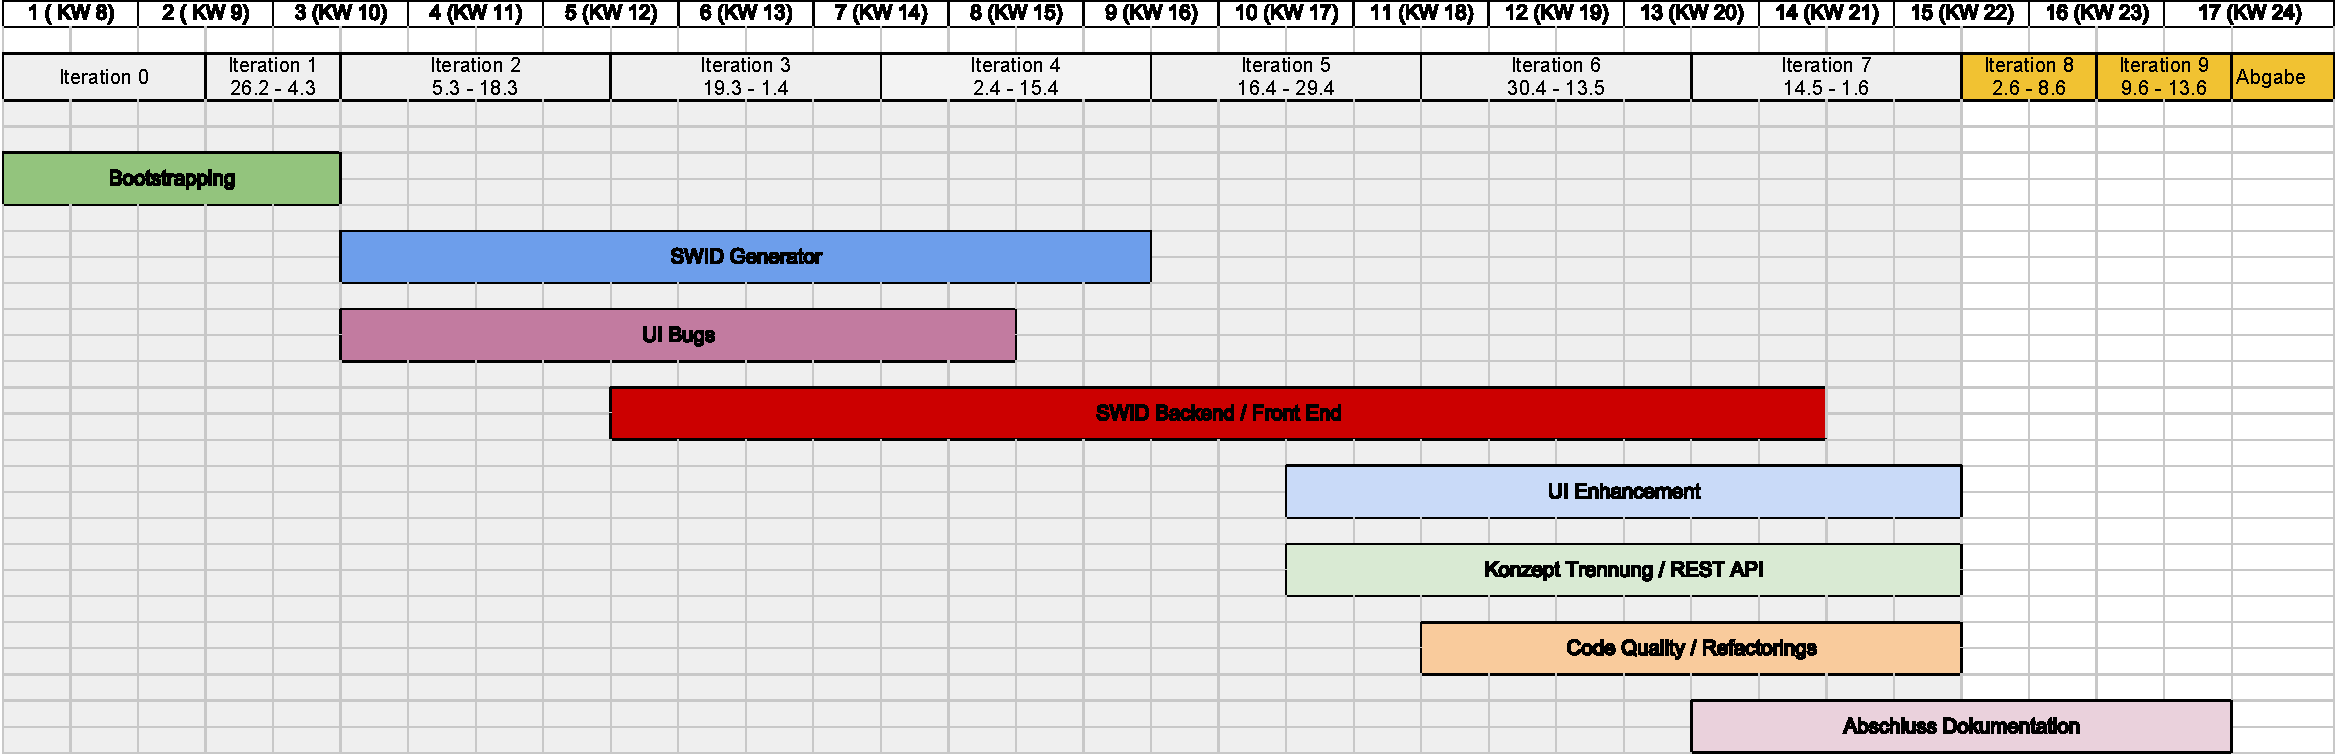
\includegraphics[width=\linewidth]{images/zeitplanung/iteration_8}
		\caption{Zeitplanung zum Schluss der Arbeit}
		\label{zeitanalyse:nachher}
	\end{minipage}

\end{sidewaysfigure}


\section{Persönliche Berichte}
\label{anhang:berichte}
\subsection{Danilo Bargen}

Das Thema der vorliegenden Bachelorarbeit hat mir sehr zugesagt. Einerseits
interessiere ich mich für Security-Themen und habe deshalb bereits während dem
Studium alle Module zu Informationssicherheit an der HSR besucht. Andererseits
habe ich bereits mehrere Jahre Entwicklungserfahrung mit Python und dem
Django-Framework, das kam mir natürlich sehr entgegen.

Sehr gefreut habe ich mich auch darüber, dass es möglich war, die Arbeit zu
dritt mit meinen Mitstudenten Christian und Jonas durchzuführen. Dadurch, dass
wir in der Vergangenheit bereits mehrere Arbeiten erfolgreich zusammen
abgeschlossen haben, waren wir bereits ein eingespieltes Team und die
Zusammenarbeit klappte reibungslos. An dieser Stelle möchte ich ihnen ein
grosses Dankeschön aussprechen für die gemeinsame Zeit. \\
Auch unseren beiden Betreuern -- Prof. Dr. Andreas Steffen und Tobias Brunner --
möchte ich meinen Dank aussprechen für die gute Begleitung unserer Arbeit.

Leider verlief diese Bachelorarbeit nicht ganz ohne Hindernisse. In der vierten
Semesterwoche zog ich mir an meiner praktischen Gleitschirm-Brevetprüfung einen
komplizierten Ellbogenbruch zu, worauf ich zwei Wochen im Kantonsspital St.
Gallen verbringen musste. Zudem konnte ich auch während der zwei darauffolgenden
Wochen aufgrund der Operationswunde eine Tastatur nur einhändig bedienen.\\
Glücklicherweise konnten wir uns im Entwicklungs-Team gut mit der Situation
arrangieren. Während des Spitalaufenthaltes konnte ich über einen Tablet
Computer Code Reviews durchführen und später klappte auch das einhändige
Programmieren nach kurzer Eingewöhnungszeit relativ gut.

Obwohl wir zuletzt noch mehrere Nachtschichten einlegen mussten um unseren
Ansprüchen an die Dokumentation zu genügen, blicke ich positiv auf die
vergangene Zeit zurück und hoffe, dass die geleistete Arbeit nicht vergebens
war, sondern dass die resultierenden Softwareprodukte auch wirklich erfolgreich
in der Praxis eingesetzt werden können.



\subsection{Christian Fässler} 
An erster Stelle möchte ich bei meinen Teamkollegen Jonas Furrer und Danilo
Bargen für die super Zusammenarbeit und ihr Engagement bedanken. Da wir in
dieser Zusammensetzung bereits einige Arbeiten umgesetzt haben, waren die
Voraussetzungen für diese Arbeit optimal! Entsprechend erfolgreich war auch die
Zusammenarbeit und die gegenseitige Unterstützung.\\ Herzlichen Dank auch an die
Betreuer Prof. Dr. Andreas Steffen und Tobias Brunner für die gute Betreuung der
Arbeit. Durch die wertvollen und zeitnahen Feedbacks hatte ich stets den
Eindruck, dass unsere Arbeit sehr geschätzt wurde.

Zu Beginn der Arbeit war Danilo Bargen wegen eines Unfalls leider während 2
Wochen im Spital. Durch das eingespielte Team war dies kein Problem und wir
konnten uns schnell arrangieren.

Im Rahmen des Aufbaustudiums habe ich die Sicherheitsmodule an der HSR besucht.
Deshalb hat mir das Thema dieser Arbeit sehr zugesagt. Python-Kenntnisse konnte
ich bereits beim Start in die Arbeit mitbringen. Das Django Framework war für
mich jedoch komplettes Neuland. Spannend an dieser Arbeit war die Mischung aus
dem Entwickeln einer kompletten Standalone-Anwendung (SWID-Generator) und dem
Erweitern einer bestehenden Applikation. Ich bin sehr zufrieden mit dem
erreichten Resultat. Umso schöner finde ich es, dass es sich um ein Produkt
handelt, welches voraussichtlich auch in der Praxis eingesetzt wird.

Ich hoffe, mit den Ergebnissen unserer Arbeit hilfreiche Grundlagen für
weitergehende Arbeiten liefern zu können.


\subsection{Jonas Furrer} 



\enquote{Endpoint Compliance Monitoring based on Software Identification Tags}, dieses Thema klingt spannend, doch zu Beginn dieser Bachelorarbeit konnte ich mir noch nichts genaues darunter vorstellen. Nach einem Gespräch mit Prof. Dr. Steffen wurde klar in welche Richtung die Arbeit gehen würde.\\
Wir hatten die Gelegenheit eine Applikation 

Wir hatten die Gelegenheit uns einen
Bereich einzuarbeiten wo noch vieles offen ist. Damit begann die Einarbeitung in
die diversen Themen rund um Graphentheorie und deren Phänomene, Musiktheorie,
Mathematik und die Arbeit mit Wolfram Mathematica. Nach einer kurzen
Einarbeitungszeit konnten bereits erste Ergebnisse erzielt werden, doch mit den
Ergebnissen kam auch die Erkenntiss, dass weder das Themengebiet noch die
Grenzen der Arbeit klar abzustecken sind. Mit dieser Tatsache hatte ich zu
beginn Mühe, ich bin es mir Gewohnt Lösungsorientiert zu arbeiten. Diese Aufgabe
forderte aber einen Problemorientierten Ansatz. Als ich erkannte, dass wir nicht
auf \enquote{eine richtige} Lösung hin arbeiten, sondern darauf, das Problem zu
erkennen und wege zu einer Lösungsmöglichkeit zu finden, betrachtete ich die
Arbeit aus einer anderen Perspektive und konnte offener an die Problemstellung
heran gehen. Durch diese offene Herangehensweise kam mit jeder Idee ein neues
Problem, und mit jedem Problem zwei neue Ideen. Wir mussten uns auf einige Ideen
einschränke und diese genauer betrachten. Es fiel mir nicht einfach
Eintscheidungen zu treffen, da man nie genau sagen konnte ob eine Idee oder
deren Ergebnisse richtig oder falsch sind. Die Arbeit hat durch das grosse
Potential des Themengebietes noch viele Bereich die Vertieft werden konnten. Wir
hatten nicht die Zeit alle Ideen und Ansätze umzusetzen, einige Möglichkeiten
und Anätze konnte ich erst gegen Ende der Arbeit erkennen, da anfangs das
Grundwissen fehlte. Ich konnte von dieser Arbeit in vielerlei Hinsicht
profitieren: Ich hatte die Glegenheit mich in ein interessantes Themengebiet
einzuarbeiten und neue Werkzeuge auszuprobieren, ich habe eine für mich
ungewohnte Herangehensweise für Projekte erlebt, von den Diskusionen mit
Christian Fässler und Prof. Stoop konnte ich stets profitieren.

